\documentclass{article}
\usepackage[T1]{fontenc}
\usepackage{microtype}
\usepackage{graphicx}
\usepackage{booktabs}
\usepackage{hyperref}
\newcommand{\theHalgorithm}{\arabic{algorithm}}
\usepackage{icml2026}
\usepackage{amsmath,amssymb,amsthm,mathtools}
\usepackage{tikz}
\usetikzlibrary{arrows.meta,positioning}
\usepackage{longtable}
\usepackage{listings}
\usepackage[capitalize,noabbrev]{cleveref}
\theoremstyle{plain}
\newtheorem{theorem}{Theorem}[section]
\newtheorem{lemma}[theorem]{Lemma}
\newtheorem{proposition}[theorem]{Proposition}
\newtheorem{corollary}[theorem]{Corollary}
\theoremstyle{definition}
\newtheorem{definition}[theorem]{Definition}
\newcommand{\F}{\mathbb F_2}
\newcommand{\wt}{\operatorname{wt}}
\newcommand{\rank}{\operatorname{rank}}
\newcommand{\dist}{\delta}
\newcommand{\dopt}{d_2}
\newcommand{\E}{\mathcal E}
\icmltitlerunning{AI-Assisted Code Nonexistence Proofs}
\icmlkeywords{AI-assisted mathematics, coding theory, computational proof, formal verification}
\begin{document}
\twocolumn[
\icmltitle{AI-Assisted Nonexistence Proofs for\ Five Binary Linear Code Parameters}
\begin{icmlauthorlist}
\icmlauthor{Anonymous Authors}{anon}
\end{icmlauthorlist}
\icmlaffiliation{anon}{Anonymous Institution}
\icmlcorrespondingauthor{Anonymous Author}{anonymous@example.invalid}
\vskip 0.3in
]
\printAffiliationsAndNotice{}
\begin{abstract}
We present an AI-assisted mathematical investigation excluding binary linear codes with parameters $[43,10,\ge17]$, $[44,10,\ge18]$, $[44,11,\ge17]$, $[45,11,\ge18]$, and $[42,16,\ge13]$.
The main proof reduces the first target to extending one of 172 classified $[40,7,18]$ codes and rules out every extension through complete coset enumeration and pairwise incompatibility certificates.
Two independently implemented scans examine $2^{32}$ cosets per mother code and agree on all 429,024 accepted cosets; a separate checker replays 619,053,789 pair rejections.
Three targets follow by puncturing and shortening, while the fifth follows from a published $[41,14,14]$ nonexistence theorem.
Explicit constructions yield four exact optimal distances and the interval $16\le\dopt(45,11)\le17$.
We describe the recorded contributions of AI to exploration and verification design, and formalize the mathematical reductions in Lean with explicit interfaces for published and computational inputs.
\end{abstract}
\section{Introduction}
A binary linear code is a subspace of $\F^n$. Determining the largest possible minimum distance at fixed length and dimension is a finite problem, but a negative answer must cover every subspace, including those far from familiar constructions. A failed search for a generator matrix supplies no such coverage. This makes code nonexistence a useful setting for studying how AI-assisted mathematical work can produce independently checkable results.

We study five parameter targets through two proof routes. The main route starts with a hypothetical $[43,10,\ge17]$ code. Parity extension, a low-weight dual-word argument, and shortening force a full-support $[40,7,18]$ subcode. A published classification then reduces the unrestricted existence question to 172 concrete mother codes. Each mother has $2^{32}$ even cosets to examine. The successful reduction is stronger than an unsuccessful extension search: every pair of distinct admissible cosets is incompatible, so the three cosets required for an extension cannot exist.

The second route illustrates a different useful outcome of AI-assisted research. An apparent target, $[42,16,\ge13]$, is already excluded by a short consequence of a published theorem. Parity extension and two shortenings produce a $[41,14,\ge14]$ code; an exact-distance normalization connects it to the published exclusion of $[41,14,14]$. The contribution here is the explicit, checked connection to the requested target.

\begin{table}[t]
\caption{Five excluded targets and the resulting optimum information. Lower bounds use explicit matrices. The first three exact values and the fourth upper bound share one main proof; the last row is a consequence of published Proposition~2.}
\label{tab:results}
\centering\small
\begin{tabular}{@{}lll@{}}
\toprule
Excluded target & Proof route &  $\dopt(n,k)$\\
\midrule
$[43,10,\ge17]$ & Main exclusion & $16$\\
$[44,10,\ge18]$ & Puncturing & $17$\\
$[44,11,\ge17]$ & Shortening & $16$\\
$[45,11,\ge18]$ & Puncturing & $[16,17]$\\
$[42,16,\ge13]$ & E3 reduction & $12$\\
\bottomrule
\end{tabular}
\end{table}

Table~\ref{tab:results} states the mathematical outcomes. The evidence accompanying them has three components: a structural proof covering arbitrary binary linear codes; concrete matrices, complete enumeration records, and rejection witnesses; and Lean proofs of the reductions with named external inputs. AI contributes to literature discovery, proof development, implementation, and review. Acceptance depends on these evidence components rather than on the model's confidence or the number of favorable reviews.

For AI-assisted mathematics, the case study highlights a specific verification issue: checking that every saved candidate is valid does not show that a search saved every valid candidate. Here that distinction led to a second complete enumeration with different coordinates and traversal. The mathematical argument, computation, and recorded AI interventions are presented together so that each claimed contribution can be assessed at its actual scope.

\section{Background and Proof Obligations}
\subsection{Notation and elementary operations}
Write $[n,k,d]$ for a $k$-dimensional binary linear code of length $n$ with minimum nonzero Hamming weight exactly $d$, and $[n,k,\ge d]$ when only a lower bound is imposed. Let $\dopt(n,k)$ be the maximum achievable distance. Zero and repeated columns are allowed throughout. A code has \emph{full support} if no coordinate is identically zero. It is \emph{even} if all its words have even weight.

Puncturing deletes coordinates. Deleting $t<d(C)$ coordinates is injective on $C$ and reduces distance by at most $t$. Shortening on a coordinate set $S$ first restricts to words zero on $S$ and then deletes $S$. If the projection onto $S$ has rank $r$, shortening reduces dimension by exactly $r$ and does not reduce minimum distance. Parity extension sends $x$ to $(x,\sum_i x_i)$ and preserves dimension. These operations apply to all codes under consideration, without a symmetry or projectivity assumption.

\subsection{Classification and computational bounds}
Classical coding theory combines general inequalities with classification near extremal parameters. The Griesmer bound gives
\begin{equation}\label{eq:griesmer}
 n\ge g_2(k,d):=\sum_{j=0}^{k-1}\left\lceil d/2^j\right\rceil
\end{equation}
for a binary linear $[n,k,\ge d]$ code \citep{griesmer1960}. For the targets considered here, the decisive information is more specific than this bound. The eight-dimensional classification of \citet{bouyukliev2000} excludes exact $[41,8,18]$. We call this input \textbf{E1}. Together with $g_2(8,19)=42$, E1 also excludes $[41,8,\ge18]$.

\citet{bouyukliev2001} classify optimal binary linear codes of dimension at most seven. The input used here, \textbf{E2}, is an upper bound of 172 coordinate-equivalence classes of full-support $[40,7,18]$ codes. Our concrete catalogue contains 172 pairwise inequivalent representatives, so E2 establishes its completeness. The distribution by hull dimension is corroborated by \citet{bouyuklieva2025}: dimensions $1,3,5$ occur $33,62,77$ times. Hull counts are a consistency check; completeness follows from the class bound and actual inequivalence, not from matching these three numbers.

A separate classification technique extends residual codes. \citet{bouyuklieva2020}, Proposition~2, prove that a binary linear $[41,14,14]$ code does not exist. We call this input \textbf{E3}. Our fifth result imports the proposition as a whole and supplies the reduction from $[42,16,\ge13]$. The historical classification computations underlying E1--E3 remain published inputs; our computations concern the new extension obstruction and the explicit lower-bound matrices.

\subsection{Constructions, certification, and formal proof}
Code tables organize lower constructions and upper bounds at fixed parameters \citep{grasslTables}. They are useful starting points for identifying targets and recovering witnesses. A table entry, however, plays a different role from an explicit construction: the latter can be checked by row reduction and enumeration of all nonzero messages. We include the actual lower-bound generators in the appendix, including matrices reconstructed from the quasicyclic constructions recorded by CodeTables.

Computational nonexistence requires a finite domain with a justified connection to every hypothetical object. In the main proof, the classification fixes the mothers and a linear quotient fixes the coset domain. Two complete enumerators address coverage; a separate witness checker addresses rejection validity. These tasks are logically different. The rejected pairs have small witnesses, but the completeness of the accepted-coset lists still depends on exhaustive enumeration.

Lean~4 provides a further level of verification for definitions and deductions \citep{lean2021}; the formal developments use mathlib \citep{mathlib2020}. The formal statements refer to actual finite-dimensional subspaces, weights, and generator matrices. Their external hypotheses identify the precise facts supplied by published classification and computational evidence. This arrangement exposes where formal proof ends and ordinary computational trust begins, while checking the entire intervening mathematical argument.

\section{From an Arbitrary Code to 172 Mothers}
\label{sec:reduction}
\begin{theorem}\label{thm:main}
There is no binary linear $[43,10,\ge17]$ code.
\end{theorem}
The proof uses E1 and E2 together with the finite computation specified in Section~\ref{sec:computation}. We give the full structural argument here; Appendix~\ref{app:algebra} supplies the auxiliary identities and coordinate details.

\subsection{A forced dual word of weight four}
Suppose that $C_0$ is a $[43,10,\ge17]$ code. Its parity extension $C$ is an even $[44,10,\ge18]$ code: an odd weight at least 17 increases by one, and an even weight at least 17 is already at least 18. Conversely, puncturing any coordinate of an even $[44,10,\ge18]$ code gives a $[43,10,\ge17]$ code. Thus it suffices to exclude $C$.

\begin{lemma}\label{lem:three}
Every three columns of a generator matrix for $C$ are linearly independent.
\end{lemma}
\begin{proof}
If three columns had rank at most two, shortening on them would give a length-41 code of dimension at least eight and distance at least 18. Taking an eight-dimensional subcode contradicts E1, since the Griesmer bound excludes distance at least 19.
\end{proof}
Let $A_w$ and $B_j$ count weight-$w$ words of $C$ and weight-$j$ words of $C^\perp$, respectively. Lemma~\ref{lem:three} implies $B_1=B_2=B_3=0$. Define the length-44 binary Krawtchouk polynomials by
\[
 K_j(w)=\sum_{t=0}^j(-1)^t\binom wt\binom{44-w}{j-t}.
\]
The MacWilliams identities give $\sum_w A_w K_j(w)=2^{10}B_j$. Consider
\begin{align}
 P(w)&=(w-18)(w-20)(w-24)(w-26)\notag\\
 &=\tfrac32K_4(w)+22K_2(w)+\tfrac{403}{2}K_0(w).
 \label{eq:polynomial}
\end{align}
Every allowed nonzero weight is even and at least 18, so $P(w)\ge0$ on these weights. Since $P(0)=224640$ and $B_0=1$,
\[
 224640\le\sum_w A_wP(w)=1536B_4+206336.
\]
Therefore $B_4\ge143/12$, hence $B_4\ge12$. In particular, $C^\perp$ contains a weight-four word.

\subsection{Shortening gives a full-support mother}
\begin{lemma}\label{lem:mother}
Shortening $C$ on the support of a weight-four dual word produces an even full-support $[40,7,18]$ code $K$.
\end{lemma}
\begin{proof}
Permute the four support coordinates to the end. Their generator columns $v_1,v_2,v_3,v_4\in\F^{10}$ satisfy $v_1+v_2+v_3+v_4=0$. Any three are independent, so the projection rank is three. Shortening therefore has dimension $10-3=7$, length 40, and distance at least 18. All its words remain even. If its distance exceeded 18, it would be at least 20, contradicting $g_2(7,20)=42>40$.

Let $U=\langle v_1,v_2,v_3\rangle$. A remaining coordinate would vanish on every shortened word precisely if its generator column belonged to $U$. The seven nonzero vectors of $U$ are the four support columns and their three distinct pair sums. An outside column equal to a support column would give a dependent pair; an outside column equal to a pair sum would give a dependent triple. The zero vector is also excluded by Lemma~\ref{lem:three}. Thus no outside coordinate vanishes, and $K$ has full support.
\end{proof}
By E2 and the verified inequivalence of the 172 actual representatives, $K$ is coordinate-equivalent to one catalogue member. A permutation of its 40 coordinates preserves every distance condition below.

\subsection{Every extension requires compatible cosets}
Choose a basis for the shortened subcode and extend it to a basis of $C$. The image on the final four coordinates is the even-weight subspace of $\F^4$: it has dimension three and is orthogonal to $(1,1,1,1)$. A change of row basis gives
\begin{equation}\label{eq:normal}
 G_C=\begin{pmatrix}
 G_K&0000\\
 a_1&1001\\
 a_2&0101\\
 a_3&0011
 \end{pmatrix}.
\end{equation}
The $a_i\in\F^{40}$ have even weight because $C$ is even. For a vector $a$, set $\dist_K(a)=\min_{c\in K}\wt(a+c)$. Each nonzero combination of one or two of the final three rows has tail weight two; the combination of all three has tail weight four. Consequently the distance condition for \eqref{eq:normal} is exactly
\begin{align}
 \dist_K(a_i)&\ge16 &&(1\le i\le3),\notag\\
 \dist_K(a_i+a_j)&\ge16 &&(i<j),\label{eq:extension}\\
 \dist_K(a_1+a_2+a_3)&\ge14.\notag
\end{align}

Let $E_{40}$ be the even-weight subspace of $\F^{40}$. Since $K\subset E_{40}$, the quotient $E_{40}/K$ has dimension $39-7=32$. Let $F_K$ consist of the cosets satisfying $\dist_K(a)\ge16$. Join distinct cosets $a+K,b+K\in F_K$ when $\dist_K(a+b)\ge16$. Conditions~\eqref{eq:extension} require a triangle in this graph; the three cosets must be distinct because equal cosets have sum-distance zero. The computation finds that all 172 graphs have no edges. This stronger obstruction rules out \eqref{eq:normal} before the triple-sum condition is needed, proving Theorem~\ref{thm:main}.

\section{Complete Enumeration and Rejection Certificates}
\label{sec:computation}
The computational statement used in Theorem~\ref{thm:main} is finite and explicit:
\begin{proposition}[Computed incompatibility]\label{prop:computed}
For each of the 172 catalogue codes $K$, and all distinct cosets $a+K,b+K$ with $\dist_K(a),\dist_K(b)\ge16$, one has $\dist_K(a+b)<16$.
\end{proposition}
Its verification has three parts: validating the catalogue, enumerating the complete $F_K$, and rejecting every unordered pair from that set.

\subsection{Concrete objects and canonical representatives}
For each mother, seven 40-bit integers specify the generator rows. Enumerating all 128 messages checks the rank, evenness, minimum distance 18, and full support. The 172 matrices have 21,844 nonzero messages in total. Coordinate equivalence is tested using a colored incidence graph with 40 coordinate vertices and 128 codeword vertices. Edges record the 1 entries of codewords and the two vertex types have distinct colors. Isomorphisms of these graphs correspond exactly to coordinate equivalences of the codes. The stored canonicalization results distinguish all 172 graphs.

To enumerate cosets, put a generator of $K$ into systematic form with pivot positions $p_1,\ldots,p_7$ and rows $r_1,\ldots,r_7$. The linear map
\begin{equation}\label{eq:normalizer}
 N_K(x)=x+\sum_{i=1}^7 x_{p_i}r_i
\end{equation}
zeros all pivots, has kernel $K$, and preserves parity. It gives a unique zero-pivot representative of each coset. Among the 33 free coordinates, the evenness equation removes one degree of freedom. Thus the scan domain has exactly $2^{32}$ elements, rather than a sampled or symmetry-restricted subset.

\subsection{Two implementations cover the entire domain}
The first scanner splits the 33 free bits into 27 high bits and six low bits. For each high assignment, it intersects 64-bit masks expressing the 128 distance constraints. Parity leaves 32 low assignments, so $2^{27}\cdot32=2^{32}$ even representatives are considered. An affine permutation with odd multiplier reorders the high assignments bijectively. Mask rejection is exact: a bit survives precisely when the corresponding representative has distance at least 16 from every codeword.

The second scanner constructs systematic pivots in the opposite order, builds a different basis for the 32-dimensional even quotient, and enumerates it in Gray-code order. It computes weights on actual 40-bit words against all 128 actual codewords. Early termination rejects a candidate only after a recomputed distance below 16. Its output is converted to the first normalization and compared as a complete set, not only by cardinality. All 172 sets agree.

\begin{table}[t]
\caption{Recorded complete computation. A coset visit is one element of the explicitly defined even quotient. Pair replay checks saved witnesses and does not repeat the coset scans.}
\label{tab:compute}
\centering\small
\begin{tabular}{@{}lr@{}}
\toprule
Quantity & Count\\
\midrule
Full-support mother codes & 172\\
Cosets per mother, per scanner & $2^{32}$\\
Cosets across mothers, per scanner & 738,734,374,912\\
Accepted cosets, $\sum_K|F_K|$ & 429,024\\
Unordered pairs, $\sum_K\binom{|F_K|}{2}$ & 619,053,789\\
Compatible pairs & 0\\
Replayed pair witnesses & 619,053,789\\
Invalid or nonrejecting witnesses & 0\\
\bottomrule
\end{tabular}
\end{table}

\subsection{Independent replay of every rejected pair}
Order each complete list $F_K$. For every $i<j$, the certificate stores a message $u\in\{0,\ldots,127\}$ such that
\begin{equation}\label{eq:witness}
 \wt(a_i+a_j+uG_K)<16.
\end{equation}
An independent checker reconstructs $uG_K$ from the literal generator rows, verifies the inequality, checks that the number and order of pairs are correct, and requires exact end-of-file. It also checks every saved member of $F_K$ against all 128 codewords, totaling 54,915,072 distance evaluations. The unified replay processes 149 binary streams and 23 text streams and validates all 619,053,789 witnesses.

This replay would detect a false rejection or malformed stream, but it cannot detect an admissible coset omitted from both its input list and the pair stream. Completeness is supplied separately by the two full scans. Together these checks establish Proposition~\ref{prop:computed}, with the compiler, runtime, enumeration implementations, and graph canonicalizer remaining part of the computational trust boundary.

\section{Consequences and the Fifth Target}
\label{sec:consequences}
\begin{corollary}\label{cor:three}
Binary linear $[44,10,\ge18]$, $[44,11,\ge17]$, and $[45,11,\ge18]$ codes do not exist.
\end{corollary}
\begin{proof}
Puncturing a $[44,10,\ge18]$ code gives a $[43,10,\ge17]$ code, contradicting Theorem~\ref{thm:main}. Shortening a $[44,11,\ge17]$ code on any coordinate gives a length-43 code of dimension at least ten and distance at least 17; a ten-dimensional subcode gives the same contradiction. Finally, puncturing a $[45,11,\ge18]$ code gives the excluded $[44,11,\ge17]$ parameters.
\end{proof}

For the fifth target, the exact-distance convention in E3 must be respected. The following elementary lemma supplies the connection.
\begin{lemma}[Distance normalization]\label{lem:normalize}
For $k\ge1$ and $d\ge1$, existence of a binary linear $[n,k,\ge d]$ code implies existence of a binary linear $[n,k,d]$ code.
\end{lemma}
\begin{proof}
Let the original minimum distance be $D\ge d$, and choose a word of weight $D$. Puncture $D-d$ positions in its support. Since $D-d<D$, puncturing is injective. Every nonzero word retains weight at least $D-(D-d)=d$, and the chosen word attains $d$. Append $D-d$ zero coordinates to restore length $n$ without changing dimension or distance.
\end{proof}

\begin{theorem}\label{thm:42}
There is no binary linear $[42,16,\ge13]$ code.
\end{theorem}
\begin{proof}
Parity extension of a hypothetical code gives $[43,16,\ge14]$. Shortening one coordinate loses at most one dimension. Choose a 15-dimensional subcode, shorten another coordinate, and choose a 14-dimensional subcode. The result has parameters $[41,14,\ge14]$. Lemma~\ref{lem:normalize} gives exact $[41,14,14]$, contradicting E3, namely Proposition~2 of \citet{bouyuklieva2020}.
\end{proof}
The construction in this proof permits zero columns. This is consistent with both our original domain and the binary linear code domain of E3. In particular, the proof does not assume that a minimum-weight witness survives arbitrary shortening; normalization is performed after the shortening steps.

\begin{corollary}\label{cor:optima}
The optimal distances satisfy
\begin{align*}
 \dopt(43,10)&=16,&\dopt(44,10)&=17,\\
 \dopt(44,11)&=16,&\dopt(42,16)&=12,
\end{align*}
and $16\le\dopt(45,11)\le17$.
\end{corollary}
\begin{proof}
Theorems~\ref{thm:main} and~\ref{thm:42} and Corollary~\ref{cor:three} give the upper bounds. Appendix~\ref{app:lower} specifies full-rank generators of $[43,10,16]$, $[44,10,17]$, $[44,11,16]$, and $[42,16,12]$, together with their fully enumerated weight spectra. Appending a zero coordinate to the $[44,11,16]$ code gives $[45,11,16]$.
\end{proof}

\section{AI Assistance and Formal Verification}
\label{sec:ai}
\subsection{A workflow with explicit acceptance conditions}
The research used an ARIS-style workflow: a persistent formal specification, linked literature and experiment records, parallel exploration, and separate review of proposed arguments. The specification fixed the unrestricted matrix quantifiers before search. A positive candidate required full rank and a complete nonzero-message distance check; a negative conclusion required a reduction covering the entire target class. The research memory retained unsuccessful routes with their actual scope, preventing a fixed-seed exclusion from becoming a global nonexistence claim in a later session.

The final proof does not require replaying the discovery trajectory. Candidate generation, constraint-programming models, prompts, and search order guided exploration. The accepted argument uses the reductions of Section~\ref{sec:reduction}, the published class bound, and the finite evidence of Section~\ref{sec:computation}. Figure~\ref{fig:flow} shows this dependency structure.

\begin{figure}[t]
\centering
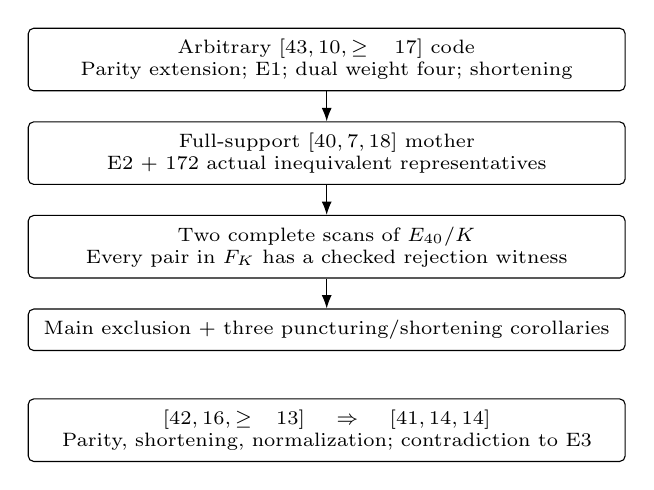
\begin{tikzpicture}[font=\scriptsize,>=Latex,
 box/.style={draw,rounded corners=2pt,align=center,text width=7.3cm,inner sep=4pt},
 node distance=3.8mm]
\node[box] (a) {Arbitrary $[43,10,\ge17]$ code\\Parity extension; E1; dual weight four; shortening};
\node[box,below=of a] (b) {Full-support $[40,7,18]$ mother\\E2 + 172 actual inequivalent representatives};
\node[box,below=of b] (c) {Two complete scans of $E_{40}/K$\\Every pair in $F_K$ has a checked rejection witness};
\node[box,below=of c] (d) {Main exclusion + three puncturing/shortening corollaries};
\node[box,below=6mm of d] (e) {$[42,16,\ge13]\ \Rightarrow\ [41,14,14]$\\Parity, shortening, normalization; contradiction to E3};
\draw[->] (a)--(b);\draw[->] (b)--(c);\draw[->] (c)--(d);
\end{tikzpicture}
\caption{Two routes to five exclusions. AI assists in finding and checking the routes. Published theorems, mathematical deductions, and explicit computations supply the proof dependencies. The fifth target uses E3 rather than the 172-mother computation.}
\label{fig:flow}
\end{figure}

\subsection{Recorded interventions and their scope}
The project records support two concrete examples of model contribution. A Gemini consultation suggested testing native early-rejection filters. The subsequent profile found that candidates in the tested instance needed about 3.38 distance checks on average before rejection, motivating further local implementation of bit-parallel low-bit masks. The implemented mask algorithm and its full-domain justification were developed in the local research process; the model's performance prediction was revised by measurement. The profile concerns an early fixed subcode, rather than the final 172-case workload.

A Grok review sharpened the missing completeness check. At that stage, independent validation established that saved cosets satisfied the constraints, while the review packet already noted that an independent full scan was missing. The review explicitly required a second implementation to decide acceptance or rejection over the entire quotient and compare complete output sets. The project then implemented the opposite-pivot, Gray-order scan described above. This intervention has a concrete consequence: it tests omitted admissible cosets, which member validation alone cannot test.

Local agents also worked on source retrieval, structural deductions, mother reconstruction, code, and proof exposition. Later consultations checked equations, quantifiers, classification scope, and evidence connections. These are documented research and review contributions. The final verification procedures operate on ordinary mathematical and computational objects and require no model API.

\subsection{What the Lean developments establish}
Both formal projects use Lean 4.34.1 and pinned mathlib. The first formalizes parity extension, puncturing, shortening, the Griesmer argument, the MacWilliams calculation, the full-support mother reduction, quotient normalization, classification coverage, and the corollaries. Actual mother matrices and lower-bound generators are connected to the abstract code definitions and checked by kernel evaluation.

The final main theorem takes four explicit parameters: E1; E2; pairwise coordinate inequivalence of the catalogue; and pair incompatibility for each catalogue member. Its type therefore records the boundary between kernel-checked deduction and the published or external computational facts. A finer interface expands the scan and certificate assumptions. The second project proves the entire reduction to exact $[41,14,14]$ and takes E3 as an explicit parameter.

The audited theorem dependencies contain the usual Lean axioms \texttt{propext}, \texttt{Classical.choice}, and \texttt{Quot.sound}, with no \texttt{sorryAx}. Explicit parameters do not appear in this axiom list. Consequently, a clean axiom audit verifies the deductions but does not discharge E1--E3, catalogue inequivalence, or the exhaustive computations. Appendix~\ref{app:formal} gives the exact interfaces.

\section{Discussion and Conclusion}
The central mechanism is a change in proof scale. An unrestricted length-43 existence question reduces to a published finite classification, then to even cosets with a precisely counted domain, and finally to low-weight witnesses for pair incompatibility. The pair obstruction is stronger than the triangle obstruction required by the extension. It makes the final rejection stage simple to replay while leaving enumeration completeness as a separate, explicit obligation.

The five targets illustrate both discovery and reuse. One main computation supplies four exclusions. A distinct literature theorem supplies the fifth through a short formalized reduction. Explicit lower constructions turn four of these upper bounds into exact values; the $[45,11]$ distance-17 question remains open in the evidence presented here.

\paragraph{Limitations.}
This is a mathematical case study, not a controlled evaluation of AI agents. The records establish specific interventions but do not isolate model effectiveness, compute savings, or an autonomous-discovery rate. Historical classification and external graph canonicalization remain trusted inputs, and the two exhaustive scanners have not been verified inside Lean. The saved pair witnesses alone cannot certify that $F_K$ is complete. Novelty or priority beyond the demonstrated statements also requires a broader literature assessment; the $[42,16]$ exclusion is presented explicitly as a consequence of the 2020 theorem.

The resulting proof package offers concrete targets for further work: replace the coset enumeration assumptions with a formally checked coverage certificate, or extend the structural method to other parameter sets. For the five targets here, the mathematical conclusions and the respective roles of AI, computation, literature, and formal deduction are fully separated and inspectable.

\label{main:end}
\section*{Impact Statement}
This work studies mathematical proof and error-correcting codes. Its methodological contribution is an auditable separation of AI-generated suggestions from the evidence used to accept a mathematical claim. The results concern finite binary linear codes; the paper does not evaluate deployment decisions or human subjects. Explicit attribution and reproducible verification reduce the risk of presenting model agreement or incomplete search as proof.
\bibliography{references}
\bibliographystyle{icml2026}
\clearpage
\appendix
\onecolumn
\section{Auxiliary Proofs and Exact Dependencies}
\label{app:algebra}
This appendix expands the mathematical ingredients used in the main text. Theorems~\ref{thm:main} and~\ref{thm:42} retain their original unrestricted code domains. E1, E2, and E3 are published inputs as specified in Section~2; Proposition~\ref{prop:computed} is the external finite computation.

\subsection{Puncturing, shortening, and parity}
For a set $S$ of $t$ coordinates, puncturing has kernel consisting of codewords supported in $S$. If $t<d(C)$, the kernel is zero, so dimension is preserved. Every remaining word loses at most $t$ ones, establishing the lower bound $d(C)-t$.

Let $\pi_S:C\to\F^S$ be coordinate projection, with rank $r$. The shortened code is the image of $\ker\pi_S$ after deleting $S$. This deletion is injective on the kernel because its members are zero on $S$. Rank-nullity gives dimension $\dim C-r$. No weight changes. For one coordinate, $r\le1$; if an exact smaller dimension is needed, choose a subspace of that dimension. This includes a coordinate that was identically zero before shortening.

Parity extension is an injective linear map because its first $n$ coordinates recover its input. Its weight is $\wt(x)$ for even-weight $x$ and $\wt(x)+1$ for odd-weight $x$. The minimum distance is therefore at least the least even integer greater than or equal to the original lower bound. Puncturing any coordinate of an even $[44,10,\ge18]$ code preserves dimension and gives distance at least 17. This proves the equivalence used at the start of Section~\ref{sec:reduction} without assuming that the punctured coordinate was originally a parity coordinate.

\subsection{A proof of the binary Griesmer bound}
For completeness, the needed inequality can be obtained by induction on dimension. Let $c\in C$ have minimum weight $D$, and puncture the $D$ positions in its support. The kernel is $\langle c\rangle$: any other nonzero word supported there has weight at least $D$ and thus equals $c$. The residual image has dimension $k-1$. For a nonzero residual word, take its two preimages $x,x+c$. If the common weight outside the support is $b$ and the weight of $x$ inside is $a$, then
\[
 a+b\ge D,\qquad D-a+b\ge D.
\]
Adding yields $b\ge\lceil D/2\rceil$. By induction,
\[
 n-D\ge\sum_{j=0}^{k-2}\left\lceil\frac{\lceil D/2\rceil}{2^j}\right\rceil
       =\sum_{j=1}^{k-1}\left\lceil\frac D{2^j}\right\rceil.
\]
The base $k=1$ is $n\ge D$. Monotonicity in $D$ gives \eqref{eq:griesmer} for a distance lower bound. In particular,
\[
 g_2(8,19)=19+10+5+3+2+1+1+1=42,
 \qquad g_2(7,20)=20+10+5+3+2+1+1=42.
\]
Both exceed 41 and 40, respectively. E1 plus the first inequality rules out distance at least 18 at parameters $(41,8)$.

\subsection{MacWilliams identity and the forcing polynomial}
For any $y\in\F^{44}$, character orthogonality gives
\[
 \sum_{x\in C}(-1)^{x\cdot y}=
 \begin{cases}2^{10},&y\in C^\perp,\\0,&y\notin C^\perp.\end{cases}
\]
In the second case, choose $x_0\in C$ with $x_0\cdot y=1$ and pair each $x$ with $x+x_0$. Summing over all $y$ of weight $j$, then interchanging two finite sums, yields
\[
 2^{10}B_j=\sum_{x\in C}\sum_{\wt(y)=j}(-1)^{x\cdot y}
 =\sum_{w=0}^{44} A_wK_j(w).
\]
For $z=44-2w$, the needed polynomials are
\[
 K_0(w)=1,\quad K_2(w)=\frac{z^2-44}{2},\quad
 K_4(w)=\frac{z^4-256z^2+5544}{24}.
\]
Substitution or direct expansion proves \eqref{eq:polynomial}. The potential negative intervals of $P(w)$ are $(18,20)$ and $(24,26)$, neither of which contains an even integer. Thus $P(w)\ge0$ at every allowed nonzero weight. Since $A_0=B_0=1$ and $B_2=0$,
\[
 \tfrac32\,2^{10}B_4+\tfrac{403}{2}\,2^{10}\ge224640,
 \qquad B_4\ge\frac{224640-206336}{1536}=\frac{143}{12}.
\]
This supplies the weight-four dual word without solving a linear program.

\subsection{Full support and the extension normal form}
The full-support claim uses the nondegenerate dot product on the message space $\F^{10}$. The shortened messages are $U^\perp$, where $U$ is the span of the four tail columns. A remaining column $v$ vanishes on all shortened messages if and only if $v\in(U^\perp)^\perp=U$. Because $\dim U=3$ and $v_4=v_1+v_2+v_3$, its nonzero vectors are exactly
\[
 v_1,v_2,v_3,v_4,\quad v_1+v_2,v_1+v_3,v_2+v_3.
\]
Each possibility contradicts independence of every three original columns, as explained in Lemma~\ref{lem:mother}. The shortening is therefore genuinely in the full-support class covered by E2.

The tail projection has kernel $K$ and image the dimension-three even subspace of $\F^4$. Choose lifts of $1001,0101,0011$ and prepend a basis for the kernel. This yields \eqref{eq:normal} by row operations, without restricting the code. For $s\in\F^3$ and $c\in K$, every word has the form
\[
 \left(c+s_1a_1+s_2a_2+s_3a_3,\ s_1(1001)+s_2(0101)+s_3(0011)\right).
\]
For $s=0$ the weight is at least 18 unless the word is zero. For $\wt(s)=1$ or 2 the tail weight is 2, and for $s=(1,1,1)$ it is 4. This proves necessity and sufficiency of \eqref{eq:extension}. Replacing an $a_i$ by a vector in its coset amounts to adding kernel rows, so all conditions depend only on cosets. A coordinate permutation of $K$ extends by the identity on the tail and preserves every condition.

\subsection{Unique even representatives and pair invariance}
In systematic form, $(r_i)_{p_j}=\delta_{ij}$. Hence $N_K(x)$ in \eqref{eq:normalizer} is zero at every pivot and $N_K(x+r_i)=N_K(x)$. Conversely, $N_K(x)=0$ implies $x=\sum_i x_{p_i}r_i\in K$. The map induces a bijection between the quotient and its zero-pivot image. Since the rows of $K$ are even, it preserves parity. On the zero-pivot subspace, evenness is the nonzero equation that the 33 free bits sum to zero; its dimension is 32. All coset and pair distances are unchanged under this normalization because $N_K(x)+x\in K$ and the map is linear.

\subsection{Distance normalization and the fifth target}
The condition $d\ge1$ in Lemma~\ref{lem:normalize} is essential to its dimension argument. If one punctured all $D$ positions of a minimum word to obtain target zero, that word would enter the kernel. For positive target $d$, only $D-d<D$ positions are removed, so no nonzero word is lost. Zero padding is permitted because our original domain is the full class of binary linear codes.

After parity extension of a hypothetical $[42,16,\ge13]$ code, two one-coordinate shortenings give dimension at least 14 and distance at least 14. Selecting a 14-dimensional subspace preserves that distance lower bound. Normalization then produces exact distance 14 at the same length and dimension. This argument discharges the exact-distance hypothesis of E3; no assertion about preserving a chosen minimum word under shortening is needed.

\section{Certificate Semantics and Reproduction}
\label{app:reproduction}
\subsection{Finite checks and completeness}
A complete checker for a mother $K$ must verify three independent properties:
\begin{enumerate}
\item The supplied matrix defines an even, full-support $[40,7,18]$ code and matches the coordinates used by the scan.
\item The list $F_K$ equals the entire set of even cosets at distance at least 16; membership and completeness are separate obligations.
\item Every unordered pair of distinct entries has a message satisfying \eqref{eq:witness}.
\end{enumerate}
The two scans provide the second property with different systematic bases and enumeration orders. The pair checker reads exactly $\binom{|F_K|}{2}$ witnesses in the declared pair order. Its weight histogram, over all mothers, is
\[
\begin{array}{c|rrrrrrr}
\text{rejection weight}&2&4&6&8&10&12&14\\\hline
\text{count}&186172&922339&4503729&16924956&61595955&171053508&363867130.
\end{array}
\]
These counts sum to 619,053,789. A message value outside $0,\ldots,127$, a missing or trailing record, a wrong matrix binding, or weight at least 16 is a verification failure.

\subsection{What is supplied with this draft}
The accompanying data directory supplies the literal mother matrices, complete per-case coverage metadata, historical pair-replay summary, and lower generators. A dependency-free script recomputes all lower spectra, mother parameters, the forcing-polynomial identity at every integer weight, and coverage counts. A separate catalogue check uses graph canonicalization for pairwise inequivalence. The local evidence map identifies the existing full scan outputs and the approximately 1.68 GB of pair-witness streams; these large streams are not embedded in the compact manuscript-source archive. Historical absolute paths in metadata are resolved against the current project root, with original records preserved.

During manuscript preparation, we rebuilt both Lean projects and reran their audits, re-enumerated every lower-bound matrix, rechecked all mother parameters and pairwise inequivalence, compared both saved accepted sets with their coordinate bindings, and replayed all 619,053,789 pair witnesses. All these checks passed. The validation log distinguishes these new checks from the original full-domain scans. Rebuilding the Lean projects or rechecking matrix spectra does not re-execute the $172\cdot2^{32}$ coset domains. Replaying all saved pair witnesses likewise does not certify that a saved list is exhaustive. Reproduction commands make these scopes explicit.

\section{Formal Interfaces and Imported Facts}
\label{app:formal}
The first project exposes the following theorem. Names are reproduced verbatim; line breaks below are typographical.
\begin{lstlisting}[basicstyle=\ttfamily\small,breaklines=true]
ECC.mainClaim_of_external_results
  (hE1 : PublishedNonexistence41)
  (hE2 : PublishedClassBound)
  (hDistinct : CatalogueInequivalent)
  (hComputed : forall i : Fin 172, PairIncompatible (catalogueCode i))
  : MainClaim
\end{lstlisting}
Here \texttt{MainClaim} means nonexistence of an actual dimension-ten subspace of $\F^{43}$ with every nonzero word of weight at least 17. E1 excludes exact $[41,8,18]$; E2 bounds the number of full-support exact $[40,7,18]$ classes. The theorem proves the connection from these hypotheses to arbitrary target codes, including the full-support reduction and actual matrix catalogue. No unproved ``catalogue reduction'' parameter remains in this final interface.

The corollary interface is \texttt{ECC.four\_table\_consequences\_of\_external\_results}. Its conclusion combines the three exact entries for $(43,10),(44,10),(44,11)$ with existence of $[45,11,\ge16]$ and nonexistence of $[45,11,\ge18]$. Kernel checks of packed matrices use \texttt{decide +kernel}. The exhaustive coset scans and graph canonicalization are external to these kernel computations.

The second project exposes
\begin{lstlisting}[basicstyle=\ttfamily\small,breaklines=true]
ECC42.reduction_42_16_to_41_14
  : CodeExists 42 16 13 -> ExactCodeExists 41 14 14
ECC42.nonexistence_of_proposition2
  : Proposition2 -> not (CodeExists 42 16 13)
\end{lstlisting}
where \texttt{Proposition2} is the published exclusion of exact $[41,14,14]$. The imported proposition is an explicit argument, not an axiom declaration. Both developments use Lean 4.34.1; their pinned manifests are included with the corresponding local projects. Audit commands inspect both final theorem types and transitive axioms, since an axiom list alone cannot reveal outstanding theorem parameters.

\section{Source Provenance and AI Attribution}
The published inputs are \citet{bouyukliev2000}, \citet{bouyukliev2001}, and Proposition~2 (printed page 179) of \citet{bouyuklieva2020}. The archived source assessment for E1 additionally locates Theorem~6.3 in Bouyukliev's doctoral thesis, and for E2 locates Table~6.2. These thesis numbering references are not journal theorem numbers. The 2025 hull paper provides a separate count cross-check. Historical classification internals are not presented as rerun computations.

The provenance records for the AI interventions retain original responses, subsequent actions, and reconciliation notes. The early Gemini profiling suggestion is connected to the native-filter experiment; the Grok completeness request is connected to the second full scan and set comparison. Later reviews are recorded as reviews of already assembled evidence. Model agreement is not included among the hypotheses of either mathematical theorem. The local record permits these specific attributions, but does not support a percentage allocation of the proof to humans or models, or a controlled comparison among systems.

\section{Explicit Lower-Bound Generators}
\label{app:lower}
In every list below, integer bit $j$ is coordinate $j$, starting from zero; message bit $i$ selects generator row $i$, and addition is XOR. The row order is the displayed order. Leading zero coordinates are retained up to the declared length. Enumeration of all $2^k-1$ nonzero messages establishes the listed exact distance; distinct message images establish rank $k$.

\subsection{The $[43,10,16]$ witness}
\begin{quote}\ttfamily\small
137539745726, 5740911900901, 3801465813127, 7302904556701,\\
3853442440940, 2103915382859, 5144838248083, 7496890689917,\\
7842576845701, 8787570300677
\end{quote}
The nonzero spectrum $(w:A_w)$ is $16:12$, $17:101$, $18:144$, $19:70$, $20:61$, $21:147$, $22:146$, $23:36$, $24:43$, $25:123$, $26:92$, $27:22$, $28:11$, $29:13$, $30:2$.

\subsection{The $[44,10,17]$ witness}
\begin{quote}\ttfamily\small
2860005872641, 5720011745283, 11440023490566, 3732392958991,\\
673493634067, 1809555608628, 204550108262, 408026474701,\\
57712634350, 114351526877
\end{quote}
The nonzero spectrum $(w:A_w)$ is $17:72$, $18:113$, $19:82$, $20:101$, $21:114$, $22:111$, $23:84$, $24:71$, $25:108$, $26:87$, $27:26$, $28:19$, $29:26$, $30:9$.

\subsection{The $[44,11,16]$ witness}
\begin{quote}\ttfamily\small
5178737328131, 10357474656262, 1218204696603, 2435335684150,\\
944061251695, 515129213098, 225190019387, 134966837980,\\
47094858883, 898731865, 514986475
\end{quote}
The nonzero spectrum $(w:A_w)$ is $16:371$, $20:880$, $24:706$, $28:88$, $32:2$.

The $[45,11,16]$ generator uses exactly the $[44,11,16]$ integers above, interpreted as 45-bit rows. Coordinate 44 is zero. Its nonzero weight spectrum is unchanged.

\subsection{The $[42,16,12]$ witness}
\begin{quote}\ttfamily\small
106065092, 139139103, 285387535, 556556412,\\
1113112824, 2195975476, 4307321038, 8653155535,\\
17229284152, 34395582853, 68730626717, 137504614505,\\
274932175173, 549758586446, 1099560464847, 2199058158699
\end{quote}
The nonzero spectrum $(w:A_w)$ is $12:675$, $16:9898$, $20:30659$, $24:21056$, $28:3161$, $32:85$, $36:1$.

\section{The 172 Actual Mothers and Their Complete Coset Counts}
\label{app:catalogue}
Each row gives the frozen zero-based catalogue index, the seven 40-bit generator rows in hexadecimal (leading zeros omitted), the hull dimension $h$, and $|F_K|$. Each pair graph has zero edges; its checked pair count is $\binom{|F_K|}{2}$. Integer bit conventions are as above. The two scans each cover $2^{32}$ cosets for every row. Hexadecimal notation specifies the full matrices rather than just invariants or equivalence-class names.
\begingroup\small
\begin{longtable}{@{}r p{12cm} r r@{}}
\caption{Literal mother generators and computed admissible-coset counts.}\\
\toprule
Index & Seven generator rows (hexadecimal) & $h$ & $|F_K|$\\
\midrule\endfirsthead
\toprule Index & Seven generator rows (hexadecimal), continued & $h$ & $|F_K|$\\\midrule\endhead
\bottomrule\endfoot
0 & \texttt{b73e546820} \texttt{ee7ca8d040} \texttt{ddf951a0c1} \texttt{bbf2a74182} \texttt{f6e74a8b04} \texttt{edce951e08} \texttt{db9f2a3430} & 5 & 668 \\
1 & \texttt{373e54d060} \texttt{ee7ca9a0c1} \texttt{5df9514182} \texttt{bbf2a68300} \texttt{f6e74b1604} \texttt{6dce943c08} \texttt{db9f2a6830} & 3 & 833 \\
2 & \texttt{b67ca8d060} \texttt{6cf951a0c1} \texttt{dff2a34182} \texttt{bbe54e8300} \texttt{75ce951604} \texttt{ef9d2a3c08} \texttt{5b3e546830} & 3 & 795 \\
3 & \texttt{b77ca8d040} \texttt{6e7951a0c1} \texttt{5df2a34182} \texttt{3be54e8304} \texttt{76ce951608} \texttt{6d9d2a3c10} \texttt{5bbe546820} & 5 & 844 \\
4 & \texttt{d3e58d3840} \texttt{afcf1270c1} \texttt{d59e2c41c2} \texttt{ab3c58a384} \texttt{dc7cb1c708} \texttt{b2f9630e10} \texttt{edf2c69c20} & 5 & 819 \\
5 & \texttt{55f2c6b081} \texttt{abe7892182} \texttt{d6cf160384} \texttt{ad9e2c4708} \texttt{5a3e58ce10} \texttt{357cb19c20} \texttt{eaf9637840} & 3 & 1334 \\
6 & \texttt{55f2c6b081} \texttt{abe7892182} \texttt{56cf164384} \texttt{ad9e2c4708} \texttt{da3e588e10} \texttt{b57cb1dc20} \texttt{6af9633840} & 3 & 1355 \\
7 & \texttt{dbe51a3081} \texttt{a7cf246182} \texttt{dd9e58c384} \texttt{ab3cb18708} \texttt{d47c634e10} \texttt{baf9c69c20} \texttt{e5f28d3840} & 5 & 867 \\
8 & \texttt{000003ffff} \texttt{0007fe99aa} \texttt{0f85382aec} \texttt{107d92e316} \texttt{26669b33d8} \texttt{455723c3e0} \texttt{84cfc3fc00} & 1 & 2578 \\
9 & \texttt{000003ffff} \texttt{0007fc7b32} \texttt{0f853a9a54} \texttt{107d92b346} \texttt{26669b2398} \texttt{455723c3e0} \texttt{84cfc3fc00} & 5 & 3930 \\
10 & \texttt{000003ffff} \texttt{0007fe95d2} \texttt{0f853ba94e} \texttt{107d930ee8} \texttt{26669bd08c} \texttt{455723e0f0} \texttt{84cfc3ff00} & 5 & 2537 \\
11 & \texttt{000003ffff} \texttt{0007fd35e8} \texttt{0f853ab942} \texttt{107d930eac} \texttt{26669bd0ce} \texttt{455723e0f0} \texttt{84cfc3ff00} & 5 & 2489 \\
12 & \texttt{000003ffff} \texttt{0007fceb52} \texttt{0f853ab186} \texttt{107d921ed8} \texttt{26669b231c} \texttt{455723c3e0} \texttt{84cfc3fc00} & 3 & 1950 \\
13 & \texttt{000003ffff} \texttt{0007fc7752} \texttt{0f853b7986} \texttt{107d922ed8} \texttt{26669bb31c} \texttt{455723c3e0} \texttt{84cfc3fc00} & 3 & 1897 \\
14 & \texttt{000003ffff} \texttt{0007fec59a} \texttt{0f853997e2} \texttt{107d9319b4} \texttt{26669a1ec8} \texttt{455723e0f0} \texttt{84cfc3ff00} & 5 & 4037 \\
15 & \texttt{000003ffff} \texttt{0007ff256c} \texttt{0f85395dd8} \texttt{107d9296e8} \texttt{26669b188e} \texttt{455723e0f0} \texttt{84cfc3ff00} & 1 & 3813 \\
16 & \texttt{000003ffff} \texttt{0007ff0d36} \texttt{0f853a7f84} \texttt{107d9329d8} \texttt{26669bb21e} \texttt{455723c3e0} \texttt{84cfc3fc00} & 5 & 4015 \\
17 & \texttt{000003ffff} \texttt{0007fd1d72} \texttt{0f8538ada8} \texttt{107d932a3c} \texttt{26669a33d0} \texttt{455723c3e0} \texttt{84cfc3fc00} & 5 & 4093 \\
18 & \texttt{000003ffff} \texttt{0007fea6b2} \texttt{0f853a6b0a} \texttt{107d90b78c} \texttt{26669b3bd0} \texttt{455723c3e0} \texttt{84cfc3fc00} & 5 & 2575 \\
19 & \texttt{000003ffff} \texttt{0007fe6734} \texttt{0f853b4a1a} \texttt{107d90b78c} \texttt{26669b3bd0} \texttt{455723c3e0} \texttt{84cfc3fc00} & 5 & 4022 \\
20 & \texttt{000003ffff} \texttt{0007ff0d3c} \texttt{0f85399632} \texttt{107d926b54} \texttt{26669bb398} \texttt{455723c3e0} \texttt{84cfc3fc00} & 5 & 4223 \\
21 & \texttt{000003ffff} \texttt{0007fd8d96} \texttt{0f853a8acc} \texttt{107d931ce8} \texttt{26669bd00e} \texttt{455723e0f0} \texttt{84cfc3ff00} & 3 & 998 \\
22 & \texttt{000003ffff} \texttt{0007ff852e} \texttt{0f85399992} \texttt{107d922dd8} \texttt{26669b321c} \texttt{455723c3e0} \texttt{84cfc3fc00} & 1 & 2036 \\
23 & \texttt{000003ffff} \texttt{0007ff8956} \texttt{0f8539ceca} \texttt{107d9293e8} \texttt{26669b1c8c} \texttt{455723e0f0} \texttt{84cfc3ff00} & 5 & 3943 \\
24 & \texttt{000003ffff} \texttt{0007fdc696} \texttt{0f853acdcc} \texttt{107d9316e8} \texttt{26669b980e} \texttt{455723e0f0} \texttt{84cfc3ff00} & 5 & 2455 \\
25 & \texttt{000003ffff} \texttt{0007fea52e} \texttt{0f8538ccca} \texttt{107d93169a} \texttt{26669b98ec} \texttt{455723e0f0} \texttt{84cfc3ff00} & 5 & 4084 \\
26 & \texttt{000003ffff} \texttt{0007fea34e} \texttt{0f853acd88} \texttt{107d93169a} \texttt{26669b98ec} \texttt{455723e0f0} \texttt{84cfc3ff00} & 5 & 4031 \\
27 & \texttt{000003ffff} \texttt{0007fdc9a6} \texttt{0f853aea0a} \texttt{107d9313b8} \texttt{26669b9ccc} \texttt{455723e0f0} \texttt{84cfc3ff00} & 1 & 2505 \\
28 & \texttt{000003ffff} \texttt{0007fd55e2} \texttt{0f853b212e} \texttt{107d9256ac} \texttt{26669b98c8} \texttt{455723e0f0} \texttt{84cfc3ff00} & 5 & 3944 \\
29 & \texttt{000003ffff} \texttt{0007fe8b74} \texttt{0f853a31be} \texttt{107d90daca} \texttt{26669b1cec} \texttt{455723e0f0} \texttt{84cfc3ff00} & 3 & 1371 \\
30 & \texttt{000003ffff} \texttt{0007ff0dcc} \texttt{0f853a66da} \texttt{107d91ab92} \texttt{26669a331c} \texttt{455723c3e0} \texttt{84cfc3fc00} & 5 & 4032 \\
31 & \texttt{000003ffff} \texttt{0007fdb0ae} \texttt{0f853ae116} \texttt{107d93265c} \texttt{2666983b98} \texttt{455723c3e0} \texttt{84cfc3fc00} & 5 & 2554 \\
32 & \texttt{000003ffff} \texttt{0007ff9136} \texttt{0f8539455a} \texttt{107d929a9c} \texttt{26669b1ce0} \texttt{455723e0f0} \texttt{84cfc3ff00} & 5 & 2505 \\
33 & \texttt{000003ffff} \texttt{0007fe953a} \texttt{0f853a3bb4} \texttt{107d90dcc6} \texttt{26669b1ee8} \texttt{455723e0f0} \texttt{84cfc3ff00} & 1 & 2264 \\
34 & \texttt{000003ffff} \texttt{0007fd53d4} \texttt{0f853a7542} \texttt{107d93869c} \texttt{26669b18e8} \texttt{455723e0f0} \texttt{84cfc3ff00} & 1 & 1908 \\
35 & \texttt{000003ffff} \texttt{0007fcaeb4} \texttt{0f853ac49a} \texttt{107d932b2c} \texttt{26669a33d0} \texttt{455723c3e0} \texttt{84cfc3fc00} & 5 & 2519 \\
36 & \texttt{000003ffff} \texttt{0007fd8f4a} \texttt{0f85395532} \texttt{107d929a5c} \texttt{26669b2398} \texttt{455723c3e0} \texttt{84cfc3fc00} & 5 & 3888 \\
37 & \texttt{000003ffff} \texttt{0007fe8f32} \texttt{0f8538e58a} \texttt{107d932a3c} \texttt{26669a33d0} \texttt{455723c3e0} \texttt{84cfc3fc00} & 5 & 2551 \\
38 & \texttt{000003ffff} \texttt{0007fe8b6a} \texttt{0f853839b2} \texttt{107d92d2cc} \texttt{26669b1cf8} \texttt{455723e0f0} \texttt{84cfc3ff00} & 5 & 2502 \\
39 & \texttt{000003ffff} \texttt{0007fd2dca} \texttt{0f85385578} \texttt{107d93989c} \texttt{26669a1ee0} \texttt{455723e0f0} \texttt{84cfc3ff00} & 3 & 971 \\
40 & \texttt{000003ffff} \texttt{0007fe8b66} \texttt{0f853a31ac} \texttt{107d90dae8} \texttt{26669b1cce} \texttt{455723e0f0} \texttt{84cfc3ff00} & 5 & 4062 \\
41 & \texttt{000003ffff} \texttt{0007fda556} \texttt{0f853ab18a} \texttt{107d93a23c} \texttt{26669b3bd0} \texttt{455723c3e0} \texttt{84cfc3fc00} & 5 & 2497 \\
42 & \texttt{000003ffff} \texttt{0007fcb972} \texttt{0f853adaa6} \texttt{107d9293cc} \texttt{26669b1cf8} \texttt{455723e0f0} \texttt{84cfc3ff00} & 3 & 1658 \\
43 & \texttt{000003ffff} \texttt{0007fd6b86} \texttt{0f827065ba} \texttt{107ad1b1d2} \texttt{2664da391c} \texttt{455763c1e0} \texttt{84cf83fe00} & 3 & 1747 \\
44 & \texttt{000003ffff} \texttt{0007ff846e} \texttt{0f827313c6} \texttt{107ad23d4a} \texttt{2664dbd98c} \texttt{455763e1f0} \texttt{84cf83fe00} & 5 & 2537 \\
45 & \texttt{000003ffff} \texttt{0007ff8a6c} \texttt{0f827315c6} \texttt{107ad2394e} \texttt{2664dbd188} \texttt{455763e1f0} \texttt{84cf83fe00} & 5 & 2592 \\
46 & \texttt{000003ffff} \texttt{0007fdb946} \texttt{0f8270e2b6} \texttt{107ad12d3c} \texttt{2664da31d8} \texttt{455763c1e0} \texttt{84cf83fe00} & 5 & 2652 \\
47 & \texttt{000003ffff} \texttt{0007fd7986} \texttt{0f827252bc} \texttt{107ad3132e} \texttt{2664db9dc8} \texttt{455763e1f0} \texttt{84cf83fe00} & 5 & 2498 \\
48 & \texttt{000003ffff} \texttt{0007fd718e} \texttt{0f8272f498} \texttt{107ad3271c} \texttt{2664dbb9d0} \texttt{455763c1e0} \texttt{84cf83fe00} & 5 & 2507 \\
49 & \texttt{000003ffff} \texttt{0007ffa45a} \texttt{0f8272f894} \texttt{107ad33338} \texttt{2664da3dc0} \texttt{455763c1e0} \texttt{84cf83fe00} & 3 & 1353 \\
50 & \texttt{000003ffff} \texttt{0007fe9a74} \texttt{0f8272d4ac} \texttt{107ad3592a} \texttt{2664db81cc} \texttt{455763e1f0} \texttt{84cf83fe00} & 3 & 1741 \\
51 & \texttt{000003ffff} \texttt{0007fd5d32} \texttt{0f8273ac54} \texttt{107ad2e986} \texttt{2664db3198} \texttt{455763c1e0} \texttt{84cf83fe00} & 3 & 1816 \\
52 & \texttt{000003ffff} \texttt{0007fc9db2} \texttt{0f82732d54} \texttt{107ad3a986} \texttt{2664da31d8} \texttt{455763c1e0} \texttt{84cf83fe00} & 5 & 2584 \\
53 & \texttt{000003ffff} \texttt{0007fd1db2} \texttt{0f82736d14} \texttt{107ad27986} \texttt{2664dbb1d8} \texttt{455763c1e0} \texttt{84cf83fe00} & 1 & 1396 \\
54 & \texttt{000003ffff} \texttt{0007ffa23c} \texttt{0f8272b954} \texttt{107ad2f186} \texttt{2664db3d98} \texttt{455763c1e0} \texttt{84cf83fe00} & 5 & 2552 \\
55 & \texttt{000003ffff} \texttt{0007fe26f4} \texttt{0f82708d7a} \texttt{107ad2b54c} \texttt{2664db3990} \texttt{455763c1e0} \texttt{84cf83fe00} & 3 & 1327 \\
56 & \texttt{000003ffff} \texttt{0007fcb3ca} \texttt{0f8273b492} \texttt{107ad324f8} \texttt{2664da391c} \texttt{455763c1e0} \texttt{84cf83fe00} & 3 & 1695 \\
57 & \texttt{000003ffff} \texttt{0007fd9734} \texttt{0f827299aa} \texttt{107ad30dcc} \texttt{2664dbd00e} \texttt{455763e1f0} \texttt{84cf83fe00} & 3 & 1633 \\
58 & \texttt{000003ffff} \texttt{0007ff839c} \texttt{0f85aad5a6} \texttt{107c9ad9c4} \texttt{2666b31ee8} \texttt{455723e0f0} \texttt{84cfc3ff00} & 3 & 1686 \\
59 & \texttt{000003ffff} \texttt{0007fcda36} \texttt{0f85a9aada} \texttt{107c99336c} \texttt{2666b23b90} \texttt{455723c3e0} \texttt{84cfc3fc00} & 3 & 1542 \\
60 & \texttt{000003ffff} \texttt{0007fed236} \texttt{0f85a9b2da} \texttt{107c9b236c} \texttt{2666b23b90} \texttt{455723c3e0} \texttt{84cfc3fc00} & 3 & 1706 \\
61 & \texttt{000003ffff} \texttt{0007fd5a96} \texttt{0f85aa2aac} \texttt{107c9bd03a} \texttt{2666b39ccc} \texttt{455723e0f0} \texttt{84cfc3ff00} & 1 & 2280 \\
62 & \texttt{000003ffff} \texttt{0007fcf326} \texttt{0f85aaa954} \texttt{107c9a8a9e} \texttt{2666b33318} \texttt{455723c3e0} \texttt{84cfc3fc00} & 1 & 1082 \\
63 & \texttt{000003ffff} \texttt{0007fd5b8a} \texttt{0f85abab1c} \texttt{107c9b321e} \texttt{2666b23fd0} \texttt{455723c3e0} \texttt{84cfc3fc00} & 1 & 1794 \\
64 & \texttt{000003ffff} \texttt{0007fd5a96} \texttt{0f81ab8b2c} \texttt{107c9ad0da} \texttt{2666b31cec} \texttt{455723e0f0} \texttt{84cfc3ff00} & 5 & 2471 \\
65 & \texttt{000003ffff} \texttt{0007ff2c5a} \texttt{0f81ab55a2} \texttt{107c9998dc} \texttt{2666b21ee0} \texttt{455723e0f0} \texttt{84cfc3ff00} & 5 & 2462 \\
66 & \texttt{000003ffff} \texttt{0007fe2db2} \texttt{0f81aa55ca} \texttt{107c9b9994} \texttt{2666b31ee8} \texttt{455723e0f0} \texttt{84cfc3ff00} & 3 & 2337 \\
67 & \texttt{000003ffff} \texttt{0007ff852e} \texttt{0f81a9b4ca} \texttt{107c9ad98c} \texttt{2666b31ee8} \texttt{455723e0f0} \texttt{84cfc3ff00} & 3 & 2481 \\
68 & \texttt{000003ffff} \texttt{0007ff1556} \texttt{0f81a97392} \texttt{107c9ba61c} \texttt{2666b23bd8} \texttt{455723c3e0} \texttt{84cfc3fc00} & 3 & 2444 \\
69 & \texttt{000003ffff} \texttt{0007ff256c} \texttt{0f81a954ba} \texttt{107c9b99c4} \texttt{2666b21ef8} \texttt{455723e0f0} \texttt{84cfc3ff00} & 5 & 4022 \\
70 & \texttt{000003ffff} \texttt{0007ff1678} \texttt{0f81aa639a} \texttt{107c9bb30c} \texttt{2666b03bd0} \texttt{455723c3e0} \texttt{84cfc3fc00} & 5 & 4054 \\
71 & \texttt{000003ffff} \texttt{0007ff153c} \texttt{0f81a97296} \texttt{107c9ba748} \texttt{2666b23b90} \texttt{455723c3e0} \texttt{84cfc3fc00} & 3 & 2765 \\
72 & \texttt{000003ffff} \texttt{0007ff499c} \texttt{0f81a92ad6} \texttt{107c9bb328} \texttt{2666b23fd0} \texttt{455723c3e0} \texttt{84cfc3fc00} & 5 & 4036 \\
73 & \texttt{000003ffff} \texttt{0007fd8db4} \texttt{0f81aab9c2} \texttt{107c9bd18c} \texttt{2666b31ee8} \texttt{455723e0f0} \texttt{84cfc3ff00} & 3 & 3022 \\
74 & \texttt{000003ffff} \texttt{0007ff0bb4} \texttt{0f81a9bac2} \texttt{107c9bd28c} \texttt{2666b21ce8} \texttt{455723e0f0} \texttt{84cfc3ff00} & 3 & 1957 \\
75 & \texttt{000003ffff} \texttt{0007ff1674} \texttt{0f863a67b2} \texttt{107e38b558} \texttt{2666d3399c} \texttt{455763c1e0} \texttt{84cf83fe00} & 1 & 3260 \\
76 & \texttt{000003ffff} \texttt{0007fdacc6} \texttt{0f86283eb4} \texttt{107e92c9cc} \texttt{2664e30ee8} \texttt{455733f0f0} \texttt{84cfc3ff00} & 1 & 2510 \\
77 & \texttt{000003ffff} \texttt{0007feaa4e} \texttt{0f862926ba} \texttt{107e92d31c} \texttt{2664e31bd0} \texttt{455733e3e0} \texttt{84cfc3fc00} & 5 & 2458 \\
78 & \texttt{000003ffff} \texttt{0007fd966c} \texttt{0f86293b46} \texttt{107e925ab4} \texttt{2664e3a338} \texttt{455733c3c0} \texttt{84cfc3fc00} & 1 & 2211 \\
79 & \texttt{000003ffff} \texttt{0007ff84ae} \texttt{0f862aca9a} \texttt{107e931ad2} \texttt{2664e3931c} \texttt{455733e3e0} \texttt{84cfc3fc00} & 1 & 1674 \\
80 & \texttt{000003ffff} \texttt{0007fdc58e} \texttt{0f862b4ec2} \texttt{107e9256d2} \texttt{2664e398e4} \texttt{455733e0f8} \texttt{84cfc3ff00} & 5 & 2538 \\
81 & \texttt{000003ffff} \texttt{0007ff8a4e} \texttt{0f8628b8d6} \texttt{107e92d296} \texttt{2664e31ce4} \texttt{455733e0f8} \texttt{84cfc3ff00} & 3 & 2061 \\
82 & \texttt{000003ffff} \texttt{0007fe9a3a} \texttt{0f8629b686} \texttt{107e925b54} \texttt{2664e36398} \texttt{45573383e0} \texttt{84cfc3fc00} & 5 & 2498 \\
83 & \texttt{000003ffff} \texttt{0007fd36ac} \texttt{0f862b2a9a} \texttt{107e9272d2} \texttt{2664e3c31c} \texttt{45573383e0} \texttt{84cfc3fc00} & 3 & 2170 \\
84 & \texttt{000003ffff} \texttt{0007fe5aaa} \texttt{0f862874f4} \texttt{107e92ab4a} \texttt{2664e3338c} \texttt{455733c3f0} \texttt{84cfc3fc00} & 1 & 2573 \\
85 & \texttt{000003ffff} \texttt{0007fe466e} \texttt{0f874ab53a} \texttt{107ecb258a} \texttt{26655239cc} \texttt{455663c1f0} \texttt{84cf83fe00} & 5 & 2444 \\
86 & \texttt{000003ffff} \texttt{0007feb156} \texttt{0f8748d478} \texttt{107ecb198c} \texttt{2665521fd0} \texttt{455663e1e0} \texttt{84cf83fe00} & 5 & 3929 \\
87 & \texttt{000003ffff} \texttt{0007feb586} \texttt{0f8748d8b2} \texttt{107ecb1354} \texttt{2665531d98} \texttt{455663e1e0} \texttt{84cf83fe00} & 3 & 2167 \\
88 & \texttt{000003ffff} \texttt{0007fe665a} \texttt{0f874b289c} \texttt{107ecbb11e} \texttt{2665503de8} \texttt{455663c1f0} \texttt{84cf83fe00} & 3 & 1271 \\
89 & \texttt{000003ffff} \texttt{0007feb236} \texttt{0f874b14aa} \texttt{107ec9d93c} \texttt{2665521fd0} \texttt{455663e1e0} \texttt{84cf83fe00} & 5 & 2454 \\
90 & \texttt{000003ffff} \texttt{0007ff645a} \texttt{0f87492b92} \texttt{107ec9b11c} \texttt{2665523de0} \texttt{455663c1f0} \texttt{84cf83fe00} & 5 & 2564 \\
91 & \texttt{000003ffff} \texttt{0007fc567c} \texttt{0f874aa75a} \texttt{107ec935a8} \texttt{26655239cc} \texttt{455663c1f0} \texttt{84cf83fe00} & 5 & 2484 \\
92 & \texttt{000003ffff} \texttt{0007ff146e} \texttt{0f87492d38} \texttt{107eca79ca} \texttt{266553b18c} \texttt{455663c1f0} \texttt{84cf83fe00} & 5 & 3958 \\
93 & \texttt{000003ffff} \texttt{0007ff1674} \texttt{0f87498cb2} \texttt{107eca5958} \texttt{266553919c} \texttt{455663e1e0} \texttt{84cf83fe00} & 5 & 3987 \\
94 & \texttt{000003ffff} \texttt{0007fe167a} \texttt{0f87492cd8} \texttt{107ecab96c} \texttt{266553318e} \texttt{455663c1f0} \texttt{84cf83fe00} & 5 & 4047 \\
95 & \texttt{000003ffff} \texttt{0007fe5666} \texttt{0f8748d94a} \texttt{107eca938c} \texttt{2665531dd0} \texttt{455663e1e0} \texttt{84cf83fe00} & 3 & 1380 \\
96 & \texttt{000003ffff} \texttt{0007fe0eea} \texttt{0f874aad5c} \texttt{107ec8e86c} \texttt{266553318e} \texttt{455663c1f0} \texttt{84cf83fe00} & 5 & 4002 \\
97 & \texttt{000003ffff} \texttt{0007fe36e4} \texttt{0f86716a6e} \texttt{107d925cb8} \texttt{26661b90ce} \texttt{455723e0f0} \texttt{84cfc3ff00} & 3 & 3090 \\
98 & \texttt{000003ffff} \texttt{0007fe87d4} \texttt{0f8671ca4c} \texttt{107d93139a} \texttt{26661a1cec} \texttt{455723e0f0} \texttt{84cfc3ff00} & 5 & 4053 \\
99 & \texttt{000003ffff} \texttt{0007fcbca6} \texttt{0f8672c98a} \texttt{107d9391ac} \texttt{26661b1ec8} \texttt{455723e0f0} \texttt{84cfc3ff00} & 5 & 4070 \\
100 & \texttt{000003ffff} \texttt{0007ff6136} \texttt{0f8671ab5a} \texttt{107d912e78} \texttt{26661a339c} \texttt{455723c3e0} \texttt{84cfc3fc00} & 1 & 2586 \\
101 & \texttt{000003ffff} \texttt{0007fd7272} \texttt{0f8672e69a} \texttt{107d93a0dc} \texttt{26661b3b18} \texttt{455723c3e0} \texttt{84cfc3fc00} & 5 & 3978 \\
102 & \texttt{000003ffff} \texttt{0007fd8bb2} \texttt{0f86728dc8} \texttt{107d930e6c} \texttt{26661bd08e} \texttt{455723e0f0} \texttt{84cfc3ff00} & 1 & 1327 \\
103 & \texttt{000003ffff} \texttt{0007fcaeb4} \texttt{0f867156d6} \texttt{107d919a9a} \texttt{26661a1cec} \texttt{455723e0f0} \texttt{84cfc3ff00} & 5 & 2535 \\
104 & \texttt{000003ffff} \texttt{0007ff4596} \texttt{0f8671ceaa} \texttt{107d92963c} \texttt{26661b18ce} \texttt{455723e0f0} \texttt{84cfc3ff00} & 1 & 2614 \\
105 & \texttt{000003ffff} \texttt{0007ff32a6} \texttt{0f867159ba} \texttt{107d919ad8} \texttt{26661a1cec} \texttt{455723e0f0} \texttt{84cfc3ff00} & 5 & 2493 \\
106 & \texttt{000003ffff} \texttt{0007fda5b2} \texttt{0f8672a9ce} \texttt{107d930ed4} \texttt{26661bb318} \texttt{455723c3e0} \texttt{84cfc3fc00} & 1 & 2434 \\
107 & \texttt{000003ffff} \texttt{0007fe3374} \texttt{0f85b3546e} \texttt{107e5398a6} \texttt{26669a1ec8} \texttt{455723e0f0} \texttt{84cfc3ff00} & 5 & 3959 \\
108 & \texttt{000003ffff} \texttt{0007fe66a6} \texttt{0f85b0ab2a} \texttt{107e512f8c} \texttt{26669a33d0} \texttt{455723c3e0} \texttt{84cfc3fc00} & 5 & 4021 \\
109 & \texttt{000003ffff} \texttt{0007ff4556} \texttt{0f85b1598a} \texttt{107e53a23c} \texttt{26669a33d0} \texttt{455723c3e0} \texttt{84cfc3fc00} & 3 & 1673 \\
110 & \texttt{000003ffff} \texttt{0007fd8db4} \texttt{0f85b216b8} \texttt{107e53a30e} \texttt{26669b3bd0} \texttt{455723c3e0} \texttt{84cfc3fc00} & 5 & 4207 \\
111 & \texttt{000003ffff} \texttt{0007fd3a56} \texttt{0f85b14d64} \texttt{107e53918e} \texttt{26669a1ec8} \texttt{455723e0f0} \texttt{84cfc3ff00} & 5 & 3927 \\
112 & \texttt{000003ffff} \texttt{0007ff312e} \texttt{0f85b159c8} \texttt{107e519c9a} \texttt{26669a1eec} \texttt{455723e0f0} \texttt{84cfc3ff00} & 5 & 3957 \\
113 & \texttt{000003ffff} \texttt{0007fd66d2} \texttt{0f81aaa35c} \texttt{107c5af21c} \texttt{2666b33b98} \texttt{455723c3e0} \texttt{84cfc3fc00} & 5 & 4078 \\
114 & \texttt{000003ffff} \texttt{0007fdb2c6} \texttt{0f81aaa758} \texttt{107c5b361c} \texttt{2666b23b90} \texttt{455723c3e0} \texttt{84cfc3fc00} & 3 & 2023 \\
115 & \texttt{000003ffff} \texttt{0007fea746} \texttt{0f81ab0ed8} \texttt{107c5baa94} \texttt{2666b33318} \texttt{455723c3e0} \texttt{84cfc3fc00} & 3 & 913 \\
116 & \texttt{000003ffff} \texttt{0007fd9a56} \texttt{0f81abaa98} \texttt{107c5b331c} \texttt{2666b23fd0} \texttt{455723c3e0} \texttt{84cfc3fc00} & 3 & 1617 \\
117 & \texttt{000003ffff} \texttt{0007ff9256} \texttt{0f81aaa2ba} \texttt{107c593b2c} \texttt{2666b23fd0} \texttt{455723c3e0} \texttt{84cfc3fc00} & 1 & 1999 \\
118 & \texttt{000003ffff} \texttt{0007ff924e} \texttt{0f81aaa2ba} \texttt{107c593734} \texttt{2666b23bd8} \texttt{455723c3e0} \texttt{84cfc3fc00} & 1 & 3010 \\
119 & \texttt{000003ffff} \texttt{0007fdd156} \texttt{0f81aaa56c} \texttt{107c5b568a} \texttt{2666b3988c} \texttt{455723e0f0} \texttt{84cfc3ff00} & 3 & 1684 \\
120 & \texttt{000003ffff} \texttt{0007fda63c} \texttt{0f81a97386} \texttt{107c5bab50} \texttt{2666b23398} \texttt{455723c3e0} \texttt{84cfc3fc00} & 3 & 973 \\
121 & \texttt{000003ffff} \texttt{0007fde30e} \texttt{0f81ab946a} \texttt{107c5ae654} \texttt{2666b33b98} \texttt{455723c3e0} \texttt{84cfc3fc00} & 5 & 2531 \\
122 & \texttt{000003ffff} \texttt{0007fdd896} \texttt{0f81ab895c} \texttt{107c5af28a} \texttt{2666b31cec} \texttt{455723e0f0} \texttt{84cfc3ff00} & 3 & 1325 \\
123 & \texttt{000003ffff} \texttt{0007fe4d78} \texttt{0f81ab869c} \texttt{107c5af42a} \texttt{2666b318cc} \texttt{455723e0f0} \texttt{84cfc3ff00} & 3 & 2371 \\
124 & \texttt{000003ffff} \texttt{0007fe4d5c} \texttt{0f81aa86ae} \texttt{107c5b7438} \texttt{2666b398ce} \texttt{455723e0f0} \texttt{84cfc3ff00} & 5 & 3968 \\
125 & \texttt{000003ffff} \texttt{0007fd94f8} \texttt{0f8548e762} \texttt{107ea2b2ac} \texttt{2665333b30} \texttt{45563bc3c0} \texttt{84cfc3fc00} & 5 & 2654 \\
126 & \texttt{000003ffff} \texttt{0007ff859c} \texttt{0f854ad8cc} \texttt{107ea2e88e} \texttt{2665330ee8} \texttt{45563bf0f0} \texttt{84cfc3ff00} & 3 & 1605 \\
127 & \texttt{000003ffff} \texttt{0007fdc66c} \texttt{0f854ae4b2} \texttt{107ea3643a} \texttt{26653388bc} \texttt{45563bf0c0} \texttt{84cfc3ff00} & 3 & 1590 \\
128 & \texttt{000003ffff} \texttt{0007ff15a6} \texttt{0f8549555a} \texttt{107ea2a6ac} \texttt{2665333b30} \texttt{45563bc3c0} \texttt{84cfc3fc00} & 3 & 1990 \\
129 & \texttt{000003ffff} \texttt{0007fda696} \texttt{0f854b4cb8} \texttt{107ea26cac} \texttt{26653388ce} \texttt{45563bf0f0} \texttt{84cfc3ff00} & 5 & 4033 \\
130 & \texttt{000003ffff} \texttt{0007fcd9d2} \texttt{0f866a7164} \texttt{107ba39296} \texttt{2664f31ce6} \texttt{455733e0f8} \texttt{84cfc3ff00} & 5 & 2517 \\
131 & \texttt{000003ffff} \texttt{0007fe3b52} \texttt{0f866b4196} \texttt{107ba3499a} \texttt{2664f3921c} \texttt{455733e3e0} \texttt{84cfc3fc00} & 3 & 1666 \\
132 & \texttt{000003ffff} \texttt{0007fceb2c} \texttt{0f866ac156} \texttt{107ba2ca56} \texttt{2664f37398} \texttt{45573383e0} \texttt{84cfc3fc00} & 3 & 1216 \\
133 & \texttt{000003ffff} \texttt{0007fd6a36} \texttt{0f866a469a} \texttt{107ba256d2} \texttt{2664f39b1c} \texttt{455733e3e0} \texttt{84cfc3fc00} & 3 & 1524 \\
134 & \texttt{000003ffff} \texttt{0007fe4ec6} \texttt{0f8668c87a} \texttt{107ba17392} \texttt{2664f2631c} \texttt{45573383e0} \texttt{84cfc3fc00} & 5 & 3990 \\
135 & \texttt{000003ffff} \texttt{0007fe26da} \texttt{0f82f2cb48} \texttt{107b4a956c} \texttt{2664d3198e} \texttt{455763e1f0} \texttt{84cf83fe00} & 5 & 2557 \\
136 & \texttt{000003ffff} \texttt{0007feaa6a} \texttt{0f81f2d2a4} \texttt{107e8a9cb4} \texttt{2664b31ec8} \texttt{455723e0f0} \texttt{84cfc3ff00} & 5 & 3937 \\
137 & \texttt{000003ffff} \texttt{0007fdb2a6} \texttt{0f84d2a794} \texttt{107e9b3754} \texttt{26652a3b98} \texttt{455633c3e0} \texttt{84cfc3fc00} & 1 & 2003 \\
138 & \texttt{000003ffff} \texttt{0007fdc65a} \texttt{0f84d2d2ac} \texttt{107e9b40ae} \texttt{26652b9b30} \texttt{455633e3c0} \texttt{84cfc3fc00} & 5 & 2546 \\
139 & \texttt{000003ffff} \texttt{0007fcd6aa} \texttt{0f868966cc} \texttt{107eab9886} \texttt{2664b21cf8} \texttt{455723e0f0} \texttt{84cfc3ff00} & 5 & 4089 \\
140 & \texttt{000003ffff} \texttt{0007fe6aac} \texttt{0f8688f354} \texttt{107ea89b98} \texttt{2664b3231e} \texttt{455723c3e0} \texttt{84cfc3fc00} & 5 & 4361 \\
141 & \texttt{000003ffff} \texttt{0007ff893a} \texttt{0f8688eb4c} \texttt{107ea93278} \texttt{2664b23f90} \texttt{455723c3e0} \texttt{84cfc3fc00} & 1 & 2522 \\
142 & \texttt{000003ffff} \texttt{0007fe6b46} \texttt{0f868ab29a} \texttt{107ce8a71c} \texttt{2660f33b90} \texttt{455723c3e0} \texttt{84cfc3fc00} & 3 & 1956 \\
143 & \texttt{000003ffff} \texttt{0007fe98f4} \texttt{0f838aa93a} \texttt{107abb324c} \texttt{2664b23f90} \texttt{455723c3e0} \texttt{84cfc3fc00} & 3 & 1708 \\
144 & \texttt{000003ffff} \texttt{0007fd6ca6} \texttt{0f858955d8} \texttt{107d9999f4} \texttt{2666921ee8} \texttt{455723e0f0} \texttt{84cfc3ff00} & 3 & 1330 \\
145 & \texttt{000003ffff} \texttt{0007fdc33c} \texttt{0f858a96b8} \texttt{107d9b64ae} \texttt{26669398cc} \texttt{455723e0f0} \texttt{84cfc3ff00} & 3 & 1640 \\
146 & \texttt{000003ffff} \texttt{0007fdb15a} \texttt{0f858a8bd8} \texttt{107d9bd29c} \texttt{2666931ce8} \texttt{455723e0f0} \texttt{84cfc3ff00} & 1 & 2931 \\
147 & \texttt{000003ffff} \texttt{0007ff315a} \texttt{0f85894bd8} \texttt{107d9a929c} \texttt{2666931ce8} \texttt{455723e0f0} \texttt{84cfc3ff00} & 1 & 3008 \\
148 & \texttt{000003ffff} \texttt{0007fd595c} \texttt{0f8652748e} \texttt{107cb298d6} \texttt{26663b1ee8} \texttt{455723e0f0} \texttt{84cfc3ff00} & 5 & 2525 \\
149 & \texttt{000003ffff} \texttt{0007fd366a} \texttt{0f86523ab4} \texttt{107cb272d8} \texttt{26663ba31e} \texttt{455723c3e0} \texttt{84cfc3fc00} & 3 & 1762 \\
150 & \texttt{000003ffff} \texttt{0007fd8ed4} \texttt{0f83d2a964} \texttt{10795b2c66} \texttt{266563b186} \texttt{455673c1f8} \texttt{84cf83fe00} & 5 & 3768 \\
151 & \texttt{000003ffff} \texttt{0007fe5d52} \texttt{0f83e252a6} \texttt{107d32a55c} \texttt{26664b3998} \texttt{455673c1e0} \texttt{84cf83fe00} & 1 & 2676 \\
152 & \texttt{000003ffff} \texttt{0007fd9c72} \texttt{0f83e238b4} \texttt{107d332cd8} \texttt{26664bc11e} \texttt{455673f1e0} \texttt{84cf83fe00} & 3 & 1281 \\
153 & \texttt{000003ffff} \texttt{0007ff0736} \texttt{0f834b4a78} \texttt{107d325d58} \texttt{26645b919c} \texttt{455663e1e0} \texttt{84cf83fe00} & 3 & 2756 \\
154 & \texttt{000003ffff} \texttt{0007fe8cbc} \texttt{0f834a5578} \texttt{107d33984e} \texttt{26645b1f90} \texttt{455663e1e0} \texttt{84cf83fe00} & 3 & 1702 \\
155 & \texttt{000003ffff} \texttt{0007fd956c} \texttt{0f864966e2} \texttt{107c729b34} \texttt{2664ab23b8} \texttt{455733c3c0} \texttt{84cfc3fc00} & 1 & 1718 \\
156 & \texttt{000003ffff} \texttt{0007ff263c} \texttt{0f86496ae8} \texttt{107c714b56} \texttt{2664aa7398} \texttt{45573383e0} \texttt{84cfc3fc00} & 3 & 2332 \\
157 & \texttt{000003ffff} \texttt{0007ff898e} \texttt{0f8648dab8} \texttt{107c7292d6} \texttt{2664ab1ce4} \texttt{455733e0f8} \texttt{84cfc3ff00} & 3 & 2189 \\
158 & \texttt{000003ffff} \texttt{0007ff2672} \texttt{0f864aab58} \texttt{107c72b25c} \texttt{2664ab3ba0} \texttt{455733c3c0} \texttt{84cfc3fc00} & 1 & 1943 \\
159 & \texttt{000003ffff} \texttt{0007fe3a3a} \texttt{0f8708f362} \texttt{107db0d34a} \texttt{2661e3638c} \texttt{45563383f0} \texttt{84cfc3fc00} & 5 & 2566 \\
160 & \texttt{000003ffff} \texttt{0007ff8a56} \texttt{0f851929ba} \texttt{107c72d2cc} \texttt{26669b1ce0} \texttt{455723e0f0} \texttt{84cfc3ff00} & 3 & 1673 \\
161 & \texttt{000003ffff} \texttt{0007ff2a56} \texttt{0f869956da} \texttt{107ce2996c} \texttt{26654b1db0} \texttt{455673e1c0} \texttt{84cf83fe00} & 1 & 2936 \\
162 & \texttt{000003ffff} \texttt{0007ff8656} \texttt{0f8699379a} \texttt{107ce2d91c} \texttt{26654b1de0} \texttt{455673e1f0} \texttt{84cf83fe00} & 1 & 2399 \\
163 & \texttt{000003ffff} \texttt{0007fe387c} \texttt{0fe388ce96} \texttt{1719c2d32a} \texttt{2692f363cc} \texttt{446ce383f0} \texttt{85df03fc00} & 3 & 979 \\
164 & \texttt{000003ffff} \texttt{0007fec74a} \texttt{0fe30aace6} \texttt{171ba32554} \texttt{2691d3c998} \texttt{446de3f1e0} \texttt{85de03fe00} & 3 & 983 \\
165 & \texttt{03e47b9cd1} \texttt{306f897d92} \texttt{567864bf14} \texttt{1b53bf2a18} \texttt{ecc2fcb860} \texttt{0d9a86f990} \texttt{ead5d68f90} & 5 & 2570 \\
166 & \texttt{000003ffff} \texttt{0007fd529e} \texttt{0ff329a73a} \texttt{178d33322c} \texttt{266d5a3bd0} \texttt{474663c3e0} \texttt{84df83fc00} & 1 & 2700 \\
167 & \texttt{000003ffff} \texttt{0007fe4e5a} \texttt{0ff32aa866} \texttt{178d33328c} \texttt{266d5a3cf0} \texttt{474663c0f8} \texttt{84df83ff00} & 1 & 1981 \\
168 & \texttt{000003ffff} \texttt{0007fc5ea6} \texttt{0ff32b2b5a} \texttt{178d31b30c} \texttt{266d5a3f90} \texttt{474663c3e0} \texttt{84df83fc00} & 1 & 3588 \\
169 & \texttt{000003ffff} \texttt{0007fcd752} \texttt{0ff211c26a} \texttt{178c62974c} \texttt{266ea31bf0} \texttt{455f3be380} \texttt{84b7c3fc00} & 3 & 546 \\
170 & \texttt{00003fffff} \texttt{07ff866914} \texttt{0bf04bae5a} \texttt{138e730c6c} \texttt{226d63cfb0} \texttt{415b7c0fc0} \texttt{80dcfff000} & 3 & 2514 \\
171 & \texttt{ff00ff0f0f} \texttt{ffff000ff0} \texttt{fffffff000} \texttt{c5653ac566} \texttt{69c9acc6aa} \texttt{8e8eccaaa3} \texttt{f0f0f0cccc} & 3 & 3785 \\
\end{longtable}
\endgroup

\end{document}
